

\tikzset{every picture/.style={line width=0.75pt}} %set default line width to 0.75pt        

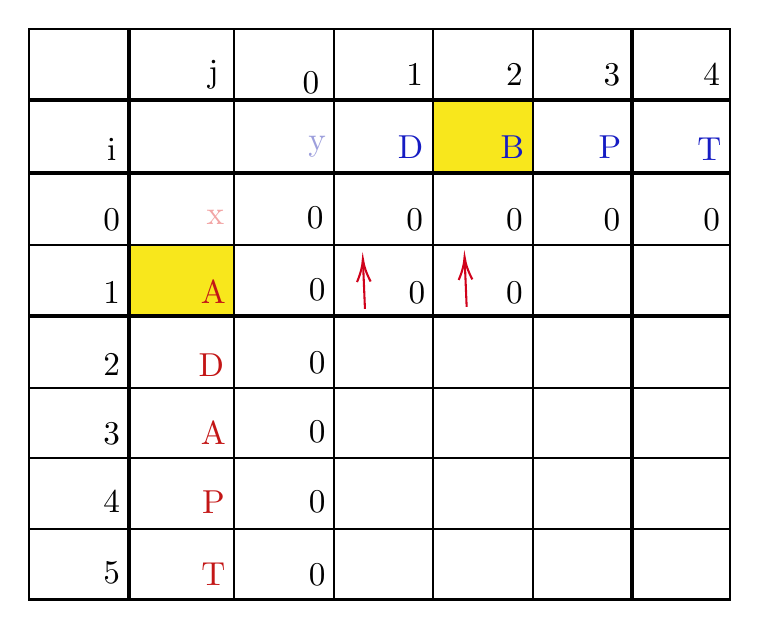
\begin{tikzpicture}[x=0.75pt,y=0.75pt,yscale=-1,xscale=1]
%uncomment if require: \path (0,396.73580169677734); %set diagram left start at 0, and has height of 396.73580169677734

\draw    (88, 46) rectangle (136, 80)   ;
\draw    (137, 46) rectangle (187, 80)   ;
\draw    (187, 46) rectangle (235, 80)   ;
\draw    (235, 46) rectangle (283, 80)   ;
\draw    (283, 46) rectangle (331, 80)   ;
\draw    (331, 46) rectangle (379, 80)   ;
\draw    (378, 46) rectangle (426, 80)   ;
\draw    (88, 81) rectangle (136, 115)   ;
\draw    (137, 81) rectangle (187, 115)   ;
\draw    (187, 81) rectangle (235, 115)   ;
\draw    (235, 81) rectangle (283, 115)   ;
\draw  [fill={rgb, 255:red, 248; green, 231; blue, 28 }  ,fill opacity=1 ]  (283, 81) rectangle (331, 115)   ;
\draw    (331, 81) rectangle (379, 115)   ;
\draw    (378, 81) rectangle (426, 115)   ;
\draw    (88, 116) rectangle (136, 150)   ;
\draw    (137, 116) rectangle (187, 150)   ;
\draw    (187, 116) rectangle (235, 150)   ;
\draw    (235, 116) rectangle (283, 150)   ;
\draw    (283, 116) rectangle (331, 150)   ;
\draw    (331, 116) rectangle (379, 150)   ;
\draw    (378, 116) rectangle (426, 150)   ;
\draw    (88, 150) rectangle (136, 184)   ;
\draw  [fill={rgb, 255:red, 248; green, 231; blue, 28 }  ,fill opacity=1 ]  (137, 150) rectangle (187, 184)   ;
\draw    (187, 150) rectangle (235, 184)   ;
\draw    (235, 150) rectangle (283, 184)   ;
\draw    (283, 150) rectangle (331, 184)   ;
\draw    (331, 150) rectangle (379, 184)   ;
\draw    (378, 150) rectangle (426, 184)   ;
\draw    (88, 185) rectangle (136, 219)   ;
\draw    (137, 185) rectangle (187, 219)   ;
\draw    (187, 185) rectangle (235, 219)   ;
\draw    (235, 185) rectangle (283, 219)   ;
\draw    (283, 185) rectangle (331, 219)   ;
\draw    (331, 185) rectangle (379, 219)   ;
\draw    (378, 185) rectangle (426, 219)   ;
\draw    (88, 219) rectangle (136, 253)   ;
\draw    (137, 219) rectangle (187, 253)   ;
\draw    (187, 219) rectangle (235, 253)   ;
\draw    (235, 219) rectangle (283, 253)   ;
\draw    (283, 219) rectangle (331, 253)   ;
\draw    (331, 219) rectangle (379, 253)   ;
\draw    (378, 219) rectangle (426, 253)   ;
\draw    (88, 253) rectangle (136, 287)   ;
\draw    (137, 253) rectangle (187, 287)   ;
\draw    (187, 253) rectangle (235, 287)   ;
\draw    (235, 253) rectangle (283, 287)   ;
\draw    (283, 253) rectangle (331, 287)   ;
\draw    (331, 253) rectangle (379, 287)   ;
\draw    (378, 253) rectangle (426, 287)   ;
\draw    (88, 287) rectangle (136, 321)   ;
\draw    (137, 287) rectangle (187, 321)   ;
\draw    (187, 287) rectangle (235, 321)   ;
\draw    (235, 287) rectangle (283, 321)   ;
\draw    (283, 287) rectangle (331, 321)   ;
\draw    (331, 287) rectangle (379, 321)   ;
\draw    (378, 287) rectangle (426, 321)   ;
\draw [color={rgb, 255:red, 208; green, 2; blue, 27 }  ,draw opacity=1 ]   (250,181) -- (249.08,159) ;
\draw [shift={(249,157)}, rotate = 447.61] [color={rgb, 255:red, 208; green, 2; blue, 27 }  ,draw opacity=1 ][line width=0.75]    (10.93,-3.29) .. controls (6.95,-1.4) and (3.31,-0.3) .. (0,0) .. controls (3.31,0.3) and (6.95,1.4) .. (10.93,3.29)   ;

\draw [color={rgb, 255:red, 208; green, 2; blue, 27 }  ,draw opacity=1 ]   (299,180) -- (298.08,158) ;
\draw [shift={(298,156)}, rotate = 447.61] [color={rgb, 255:red, 208; green, 2; blue, 27 }  ,draw opacity=1 ][line width=0.75]    (10.93,-3.29) .. controls (6.95,-1.4) and (3.31,-0.3) .. (0,0) .. controls (3.31,0.3) and (6.95,1.4) .. (10.93,3.29)   ;


\draw (177,68) node [scale=1.2] [align=left] {j};
\draw (224,72) node [scale=1.2] [align=left] {0};
\draw (274,68) node [scale=1.2] [align=left] {1};
\draw (322,68) node [scale=1.2] [align=left] {2};
\draw (369,68) node [scale=1.2] [align=left] {3};
\draw (417,68) node [scale=1.2] [align=left] {4};
\draw (128,138) node [scale=1.2] [align=left] {0};
\draw (128,173) node [scale=1.2] [align=left] {1};
\draw (128,208) node [scale=1.2] [align=left] {2};
\draw (128,241) node [scale=1.2] [align=left] {3};
\draw (128,274) node [scale=1.2] [align=left] {4};
\draw (128,308) node [scale=1.2] [align=left] {5};
\draw (178,137) node [scale=1.2,color={rgb, 255:red, 242; green, 165; blue, 165 }  ,opacity=1 ] [align=left] {x};
\draw (177,173) node [scale=1.2,color={rgb, 255:red, 195; green, 22; blue, 22 }  ,opacity=1 ] [align=left] {A};
\draw (176,208) node [scale=1.2,color={rgb, 255:red, 195; green, 22; blue, 22 }  ,opacity=1 ] [align=left] {D};
\draw (177,241) node [scale=1.2,color={rgb, 255:red, 195; green, 22; blue, 22 }  ,opacity=1 ] [align=left] {A};
\draw (177,274) node [scale=1.2,color={rgb, 255:red, 195; green, 22; blue, 22 }  ,opacity=1 ] [align=left] {P};
\draw (177,309) node [scale=1.2,color={rgb, 255:red, 195; green, 22; blue, 22 }  ,opacity=1 ] [align=left] {T};
\draw (227,103) node [scale=1.2,color={rgb, 255:red, 157; green, 159; blue, 220 }  ,opacity=1 ] [align=left] {y};
\draw (272,103) node [scale=1.2,color={rgb, 255:red, 22; green, 28; blue, 195 }  ,opacity=1 ] [align=left] {D};
\draw (321,103) node [scale=1.2,color={rgb, 255:red, 22; green, 28; blue, 195 }  ,opacity=1 ] [align=left] {B};
\draw (368,103) node [scale=1.2,color={rgb, 255:red, 22; green, 28; blue, 195 }  ,opacity=1 ] [align=left] {P};
\draw (416,104) node [scale=1.2,color={rgb, 255:red, 22; green, 28; blue, 195 }  ,opacity=1 ] [align=left] {T};
\draw (128,104) node [scale=1.2] [align=left] {i};
\draw (226,137) node [scale=1.2] [align=left] {0};
\draw (274,138) node [scale=1.2] [align=left] {0};
\draw (322,138) node [scale=1.2] [align=left] {0};
\draw (369,138) node [scale=1.2] [align=left] {0};
\draw (417,138) node [scale=1.2] [align=left] {0};
\draw (227,172) node [scale=1.2] [align=left] {0};
\draw (227,207) node [scale=1.2] [align=left] {0};
\draw (227,240) node [scale=1.2] [align=left] {0};
\draw (227,274) node [scale=1.2] [align=left] {0};
\draw (227,309) node [scale=1.2] [align=left] {0};
\draw (275,173) node [scale=1.2] [align=left] {0};
\draw (322,173) node [scale=1.2] [align=left] {0};


\end{tikzpicture}






